% !TEX root = slides.tex
\begin{frame}[t]
\label{sketch}
\vspace*{-0.3cm}

\footnotesize
\frametitle{Forward/Inverse UQ workflow}
\bi
\item \textbf{Preprocess:} Surrogate construction, GSA, select embedding
\item \textbf{Calibration:} Prior selection, MCMC
\item \textbf{Prediction:} Forward PC propagation, possible extrapolation
\ei

% !TEX root = slides.tex
\pgfdeclarelayer{background}
\pgfdeclarelayer{foreground}
\pgfsetlayers{background,main,foreground}

\normalsize

\centering
    \scalebox{0.4}{
\begin{tikzpicture}[node distance=3cm, auto, thick]
\tikzset{
   % mynode/.style={rectangle,rounded corners,draw=black, top color=white, bottom color=yellow!50,very thick, inner sep=1em, minimum size=3em, text centered,color=black},
    mynode2/.style={rectangle,rounded corners,draw=black, top color=white, bottom color=green!50,very thick, inner sep=1em, minimum size=3em, text centered,color=black},
    myarrow/.style={->, >=latex', shorten >=0pt, color=black,ultra thick}
    %,mylabel/.style={text width=7em,color=black, text centered}
}
    % We need to set at bounding box first. Otherwise the diagram
    % will change position for each frame.
    %\path[use as bounding box] (0,0) rectangle (16,8);
    \path[->]  node[mylabel, color=white] at (0,0) (init){KUKU};
\path[->] node[bigcloud, fill=brown!20, opacity=0.8, text width=30em, text height=21em] at (6.4,-0.6) (ipred) {};
\path[->] node[bigcloud, opacity=0.8, text width=32em, text height=8em] at (-0.9,2.1) (fuq) {};
\path[->] node[bigcloud, opacity=0.8, text width=43em, text height=7em] at (-0.9,-1.2) (fpred) {};

\path[->] node[bigcloud, fill=gray!20, opacity=0.8, text width=2.2em, text height=0.9em,rounded corners=2pt] at (-1.0,6.5) (fleg) {};
\path[->] node[bigcloud, fill=brown!20, opacity=0.8, text width=2.2em, text height=0.9em,rounded corners=2pt] at (-1.0,5.8) (ileg) {};

\path[->]  node[mylabel, right=-0.2 of fleg,text width=9em](fleet){Forward modeling};
\path[->]  node[mylabel, right=-0.3 of ileg,text width=9em](ilegt){Inverse modeling};

\path[->]  node[mylabel, above left=-0.8 and -2.7 of ipred](ilegt){\textbf{\emph{Calibration}}};
\path[->]  node[mylabel, below left=-0.7 and -2.7 of fuq](prep){\textbf{\emph{Preprocess}}};
\path[->]  node[mylabel, below left=-0.7 and -2.7 of fpred](postp){\textbf{\emph{Prediction}}};

\path[->] node[mynode, above right=2.8 and -1.5 of init] (model) {$f(x_i;\lambda)$};
  \path[->]                     node[mylabel, above=0.0 of model](model_label){Model};
            \path[->] node[mynode, right=2.0 of model] (sur) {$\tilde{f}(x_i;\lambda)$}
                  (model) edge [myarrow] (sur);
                 \path[->] node[mylabel, above=0.0 of sur](sur_label){Surrogate};
            \path[->] node[mynode, right=2.0 of sur] (emb) {$\tilde{f}(x_i;\lambda+\delta_{\alpha}(\xi))$};
                 \path[->] node[mylabel, above=0.0 of emb](emb_label){Embedded model}
                               (sur) edge [myarrow]  (emb);

    %\path[->] node[decision, above right=-0.2 and 0.7 of sur,text width=2.4em] (gsa) {GSA};
    \path[->]  node[mylabel, above right=-0.5 and -0.4 of sur](gsa){GSA/BF};

%                  (sur) edge [myarrow, bend left]  (gsa)
%                  (gsa) edge [myarrow, bend left]  (model);
  \path[->] node[decision, right=1.0 of emb] (lik) {Likelihood}
                  (emb) edge [myarrow]  (lik);
    \path[->] node[mynode, right=1.0 of lik] (data) {$y_i$}
                node[mylabel, above=0.1 of data](cmx){Data}
                  (data) edge [myarrow]  (lik);
   \path[->] node[mynode, below=1.6 of lik,bottom color=green!20] (post) {Posterior $p(\lambda,{\alpha}|y)$}
                  (lik) edge [myarrow] (post);
      \path[->] node[mynode, above=0.8 of lik,bottom color=green!20] (prior) {Prior $p(\lambda,{\alpha})$}
                  (prior) edge [myarrow] (lik);
       \path[->] node[mynode, left=1.3 of post] (amodel) {$h(x;\lambda+\delta_\alpha({\xi}))$}
                    node[mylabel, above=0.0 of amodel, text width=13em](amodel_label){Any QoI}
                                 (post) edge [myarrow]  (amodel);
 \path[->] node[mynode, left=1.3 of amodel,bottom color=purple!20] (ppred) {Prediction $p({h(x)}|y)$}
                  (amodel) edge [myarrow] (ppred);

  \begin{pgfonlayer}{background}
    \path (fuq.west |- ipred.north)+(-0.1,0.1) node (a) {};
    \path (fpred.east |- fpred.south)+(+2.2,-0.1) node (b) {};
    %\path[fill=blue!50!green!40!white, opacity=0.6,rounded corners]  (a) rectangle (b);
    \path[fill=white, opacity=0.6,rounded corners]  (a) rectangle (b);
    %\path[draw, black, ultra thick, rounded corners]  (a) rectangle (b);
\end{pgfonlayer}

  \end{tikzpicture}
}

\footnotesize
\bi
\item Predictive uncertainty decomposition: Total Variance = \\
\medskip
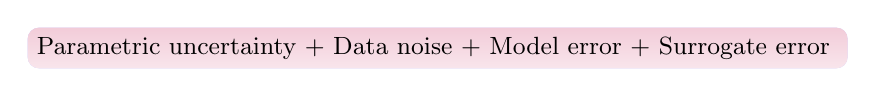
\begin{tikzpicture} \node [rounded corners,top color=purple!20, bottom color=purple!10,fill=blue!20] {
 \small{Parametric uncertainty + Data noise + Model error + Surrogate error
}
};
 \end{tikzpicture}
 \item All developments done within UQTk, lightweight C++/Python library out of SNL-CA (\emph{www.sandia.gov/uqtoolkit})
\ei

\end{frame}
